\chapter{Introduction}\label{sec:introduction}

This chapter aims to set the stage for the detailed analysis and discussion that will follow by 
providing a general overview of the problem of model robustness in 
machine learning and the current approaches to address it.

\section{The robustness challenge}\label{sec:motivation}

The field of machine learning revolves around the ambition of having computers
perform certain tasks without being programmed with task-specific instructions,
but instead by training them to find patterns in a data sample from which these 
instructions can be inferred. During training, algorithms learn from data and
experience to incrementally improve their task performance. In the process, a set
of assumptions are implicitly adopted about the statistical model generating the data 
and its connection with the desired task outcome. These assumptions constitute an 
inductive bias, and both architectures and training procedures are designed to
learn optimal biases that generalize to unseen data samples and thus lead to robust
implementations of the task at hand
\cite{p.murphyProbabilisticMachineLearning2022,m.bishopPatternRecognitionMachine2006}.
This project will focus on the assessment of the robustness of deep learning models 
performing image classification tasks.\\ 

In a broad sense, robustness can be defined as the ability of a machine learning 
model to maintain its predictive power on observations that present 
some kind of transformation or variation 
with respect to the ones used for its training
\cite{quinonero-candelaDatasetShiftMachine2009}.
Overall, three sources of variability are relevant in the context
of image classification, namely sampling randomness, adversarial
perturbations and distribution shift, which are illustrated in Figure \ref{fig:cows} 
\cite{buhmannPosteriorAgreementModel2022}.\\

Out of these, only sampling randomness is commonly accounted for by 
standard model validation techniques, in the sense that model selection 
and benchmarking are conducted using randomized subsets of unseen observations. 
In this way, the most generalizable features, and in turn the most generalizable 
models, are naturally selected. As it will be outlined in this chapter, 
this approach presents fundamental limitations
that are rooted in the very nature of deep learning models and
the data from which they learn. \\

First, the operative principles of neural networks make them vulnerable
to small perturbations in the input space, which are
often filtered out in human perception, that can lead to high-confidence
incorrect predictions \cite{szegedyIntriguingPropertiesNeural2014}.
This issue is commonly known as adversarial
vulnerability, and an ongoing arms race incentivizes the design 
of new ways of perturbing models and new ways of defending them
against such attacks. Strategies 
that foster robustness to adversarial attacks are possible, but
come at a price of hindering conventional generalization to 
sampling randomness in the original data \cite{tsiprasRobustnessMayBe2019}. \\

Second, the nature of the data used for training and selecting
models is known to influence heavily the features that the model 
will learn to be the most predictive. Lack of representativity of 
certain aspects of the data and the presence of spurious 
correlations can lead to models that generalize well to sampling 
randomness within the same dataset but that fail to do so when those 
accidental relationships are not present. This is known as an
out-of-distribution setting, given that samples in which the model is tested
are not drawn from the same probability distribution that generated
training samples \cite{quinonero-candelaDatasetShiftMachine2009}. \\

At the core of the robustness challenge lies the poor
understanding of how models construct their inductive bias and the nature
of the transformations between the space of weights and the space of 
functions that they are able to represent \cite{jimenezInductiveBiasDeep}. 
Features learned by the optimal standard classifier can be completely 
different from those learned by a robust classifier, regardless 
of the amount of data provided, which results in a fundamental limitation for task 
performance in robust models \cite{tsiprasRobustnessMayBe2019,zhangTheoreticallyPrincipledTradeoff2019}.
Besides, the feature space that deep learning models navigate is fundamentally 
different than that in which humans implicitly rely on, and we 
should therefore not expect models to be invariant to the 
same features humans are instinctively invariant to \cite{ilyasAdversarialExamplesAre2019}. \\

\begin{figure}
    \centering
    \begin{subfigure}[b]{0.22\textwidth}
        \centering
        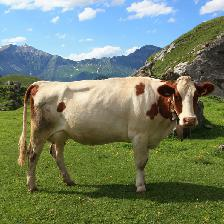
\includegraphics[width=\textwidth]{img/introduction/cow_original.jpg}
        \caption{Original}
    \end{subfigure}
    \hfill
    \begin{subfigure}[b]{0.22\textwidth}
        \centering
        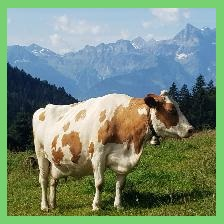
\includegraphics[width=\textwidth]{img/introduction/cow_noise.jpg}
        \caption{Sampling}
    \end{subfigure}
    \hfill
    \begin{subfigure}[b]{0.22\textwidth}
        \centering
        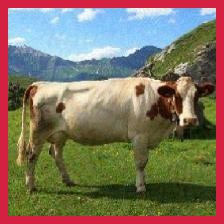
\includegraphics[width=\textwidth]{img/introduction/cow_fgsm.jpg}
        \caption{Adversarial}
    \end{subfigure}
    \hfill
    \begin{subfigure}[b]{0.22\textwidth}
        \centering
        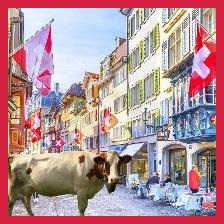
\includegraphics[width=\textwidth]{img/introduction/cow_ood.jpg}
        \caption{Distribution}
    \end{subfigure}
       \caption{Illustrative example of the three expected sources of variability. 
       A pre-trained MobileNetV2 model is shown to be vulnerable to adversarial perturbations 
       as the one represented in (c), and also to distribution shifts 
       as the one illustrated in (d), possibly because its inductive bias is influenced
       by the spurious correlation between cows and rural landscapes.}
       \label{fig:cows}
\end{figure}

This thesis will encompass all these phenomena under the same theoretical
framework, and devise a common approach to the measurement of
the shift entailed by both adversarial and distribution
variability sources. Robustness will be characterized from the space of
outcomes of the model, by means of a (posterior) probability 
distribution that will rank models and algorithms according to the
agreement in their predictions when facing different realizations of the same experiment.

\subsection{Adversarial setting}

As it was previously mentioned, certain perturbations on
original test images, which can be almost imperceptible
to the human eye, can lead to highly-confident but
incorrect predictions by deep neural networks, even when their
standard performance metrics are high.
Adversarial examples have been shown to transfer
across architectures and training procedures, and
even across subsets of data,
often yielding the same incorrect prediction in
all of these cases \cite{szegedyIntriguingPropertiesNeural2014}. \\

These intriguing phenomena were initially hypothesized to arise 
from a lack of smoothness over the input space, a property
commonly assumed in other learners, that derives from the
non-linear nature of deep learning architectures. Nevertheless,
extensive research on the field has elucidated that the root
cause is instead the linearity of its learning units, which makes them
vulnerable in certain directions of high-dimensional
spaces where small
effects can add up to significally change the outcome
\cite{goodfellowExplainingHarnessingAdversarial2015}. \\

Building on this intuition, numerous attacks have been proposed to evaluate the 
robustness of models against adversarial samples. A common strategy for inducing model 
failure involves identifying vulnerable directions in the feature space and adjusting 
perturbations to produce the desired misleading effect. Adversarial examples 
generated through these attacks can then be used to train robust models via 
regularization, thereby promoting generalization to those features present in the 
worst-case examples and thus selecting models insensitivized
to them
\cite{baiRecentAdvancesAdversarial2021}.\\

Nevertheless, adversarial learning entails decision boundaries 
that are more complex than the ones derived via standard training
(see Figure \ref{fig:adversarial_complexity}), 
intuitively demanding more data and more complex 
architectures, at the risk of
overfitting to adversarial examples themselves
\cite{schmidtAdversariallyRobustGeneralization2018}. 
These limitations express a fundamental trade-off 
that arises from the intrinsic 
disparity between robust and non-robust features
\cite{tsiprasRobustnessMayBe2019, zhangTheoreticallyPrincipledTradeoff2019}. \\

\begin{figure}
    \centering
    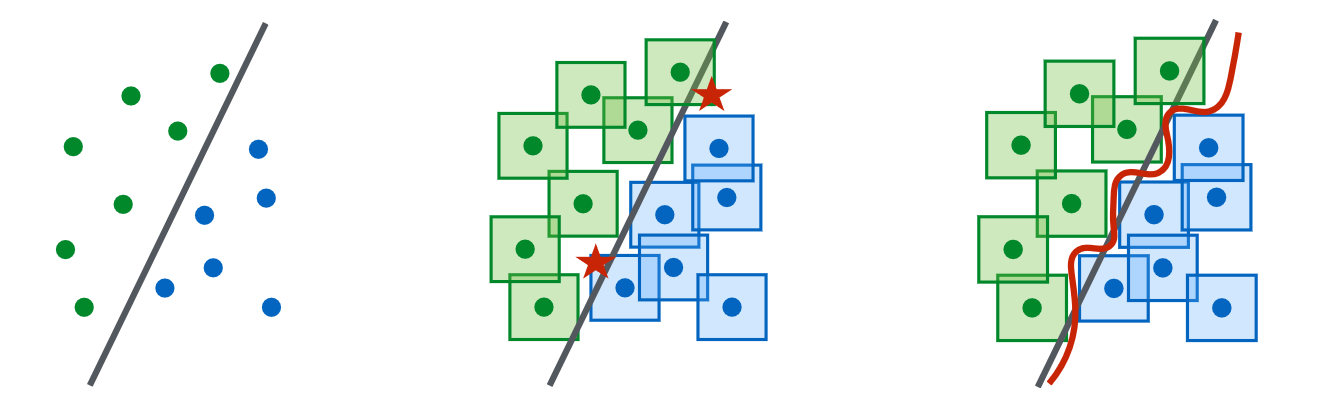
\includegraphics[width=0.65\textwidth]{img/introduction/adversarial_complexity.png}
    \caption{
    A conceptual illustration of standard vs. adversarial 
    decision boundaries. (\textbf{left}) A set of linearly-separable points. 
    (\textbf{middle}) Decision boundary learned via standard training.
    (\textbf{right}) Decision boundary learned via adversarial training.
    Both methods achieve zero training error, but only the robust model
    is able to generalize to $\ell_\infty$ perturbations.
    \cite{madryDeepLearningModels2019}
    }
    \label{fig:adversarial_complexity}
\end{figure}

Features selected via standard training
are the most predictive towards generalizing
to sampling randomness within the same dataset, but they do
not necessarily represent the features implicitly selected 
by humans and are not invariant to a human-based notion 
of similarity. Instead, features selected via adversarial training 
have been shown to better model this
invariance, and thus align much better with 
human perception, as seen in Figure \ref{fig:adversarial_loss}
\cite{ilyasAdversarialExamplesAre2019}. Furthermore, adversarial perturbations of robust 
models display salient characteristics;
that is, features that are perceived to belong to the
class they are misclassified to, as illustrated in Figure \ref{fig:salient_characteristics}
\cite{tsiprasRobustnessMayBe2019}. \\

\begin{figure}[H]
    \centering
    \begin{subfigure}[b]{0.28\textwidth}
        \centering
        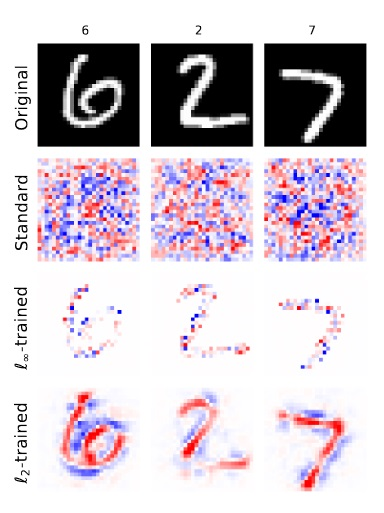
\includegraphics[width=\textwidth]{img/introduction/adversarial_loss_1.jpg}
        \caption{MNIST}
    \end{subfigure}
    \hspace{1cm}
    \begin{subfigure}[b]{0.28\textwidth}
        \centering
        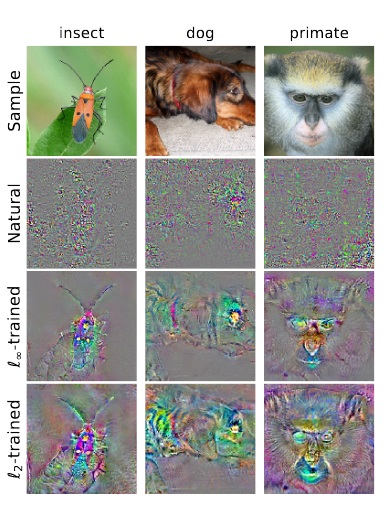
\includegraphics[width=\textwidth]{img/introduction/adversarial_loss_2.jpg}
        \caption{Restricted ImageNet}
    \end{subfigure}
       \caption{Scaled loss gradient with respect to input images.
       Input pixels yielding the highest predictive power are aligned 
       with perceptually relavant features for the case of adversarial
       models, while appearing completely random in the case of 
       standard models.
       \cite{tsiprasRobustnessMayBe2019}}
       \label{fig:adversarial_loss}
\end{figure}


\begin{figure}[H]
    \centering
    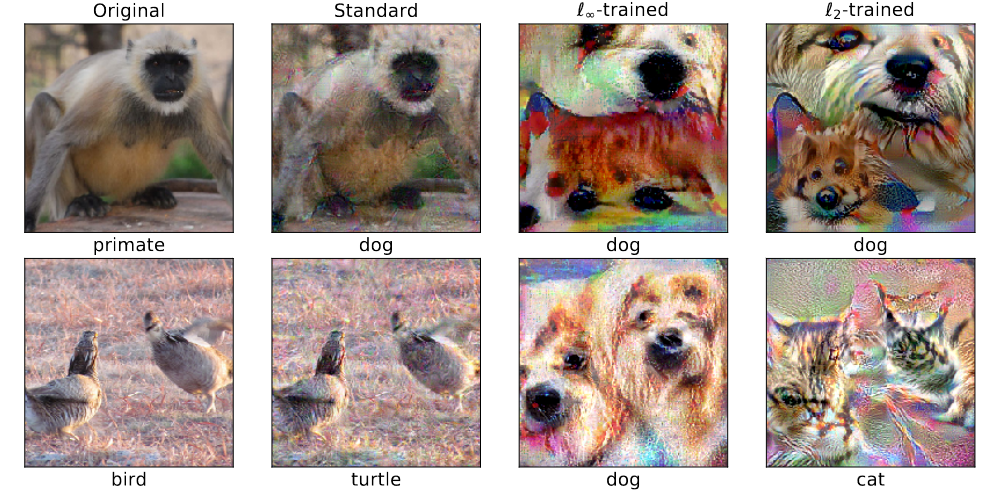
\includegraphics[width=0.45\textwidth]{img/introduction/adversarial_salient.png}
    \caption{Adversarial examples for standard and adversarially-trained models.
    Perturbed images produced for robust models 
    effectively capture salient data characteristics.
    % and appear similar to examples of a different class. 
    \cite{tsiprasRobustnessMayBe2019}}
    \label{fig:salient_characteristics}
\end{figure}

Overall, these and other findings suggest that robustness in the adversarial setting
is a fundamental property of the features that are represented by models, 
rather than of the models themselves, and the phenomenon of transferability can be
explained in these terms. Training strategies that manage to navigate the 
robustness-generalization trade-off will be the ones yielding 
the best results, provided that the data distribution
is representative of the true underlying features. 

\subsection{Out-of-distribution setting}\label{sec:intro_ood}

Most learning algorithms work under the fundamental assumption that
a causal relationship exists between input and output spaces. The target function to 
learn represents that causality and must therefore remain 
invariant regardless of the available data, which implies that 
suitable approximations of this 
function can be obtained as long as data samples are independent 
and identically distributed in the input space
\cite{muandetDomainGeneralizationInvariant2013,quinonero-candelaDatasetShiftMachine2009}. 
Nevertheless, this is not always
the case, as often real-world data does not match the same statistical
patterns of the data used for training. Ultimately, this phenomenon induces a
distribution shift that leads to poor generalization performance
\cite{zhouDomainGeneralizationSurvey2022,wangGeneralizingUnseenDomains2022,liuOutOfDistributionGeneralizationSurvey2023}. \\

\begin{figure}[h]
    \centering
    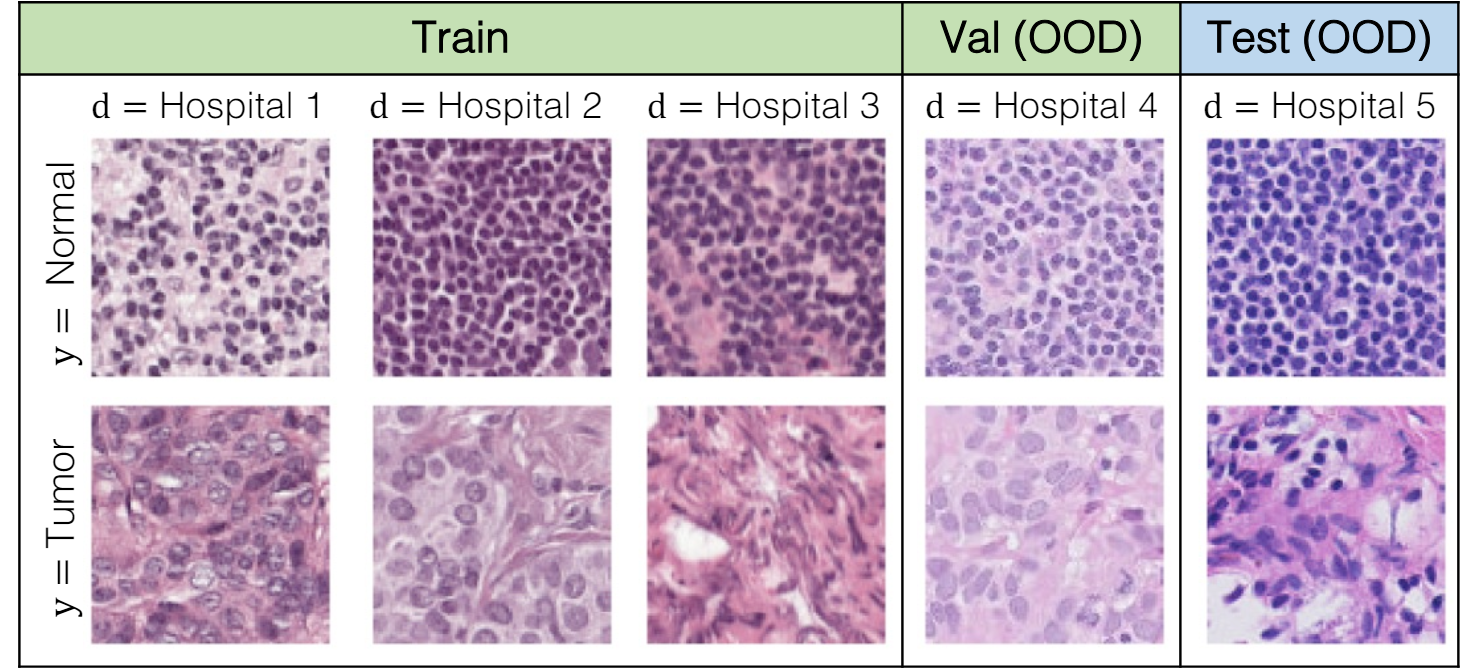
\includegraphics[width=0.5\textwidth]{img/introduction/camelyon17.png}
    \caption{The \texttt{camelyon17} (WILDS) dataset comprises images of stained 
    lymph node tissue patches sampled from different hospitals.
    \cite{kohWILDSBenchmarkIntheWild2021}
    }
    \label{fig:camelyon17}
\end{figure}

A distribution shift can arise for various reasons, namely the 
unfeasibility of collecting diverse enough data, the changing or time-dependent
nature of the data, or the implicit bias
introduced during the data collection process. This last case
is particularly relevant, as it can serve as a generalization of all
the previous cases and raise epistemological questions
about the learning framework itself. For instance, 
Figure \ref{fig:dataset_bias} refers to a cross-generalization analysis in which popular
machine learning datasets were shown to be biased towards
specific representation of features. Considering the fact that all
data is sampled from the same source (i.e. Internet), 
numerous human-induced biases are shown to determine the 
nature of representations, the most significant of all being 
negative bias, which arises when the negative subset\footnote{
    When certain observations in a dataset are labelled as belonging 
    to a specific class, the remaining observations are implicitly
    assigned to not belong to that class, and therefore define a
    negative set in the model's feature space.
}
of the dataset is not representative of the input subspace 
excluding that  particular class and results in a model that performs 
significantly worse in other datasets, even when trained with 
the same observations of that class.\\

\begin{figure}[H]
    \centering
    \begin{subfigure}[b]{0.35\textwidth}
        \centering
        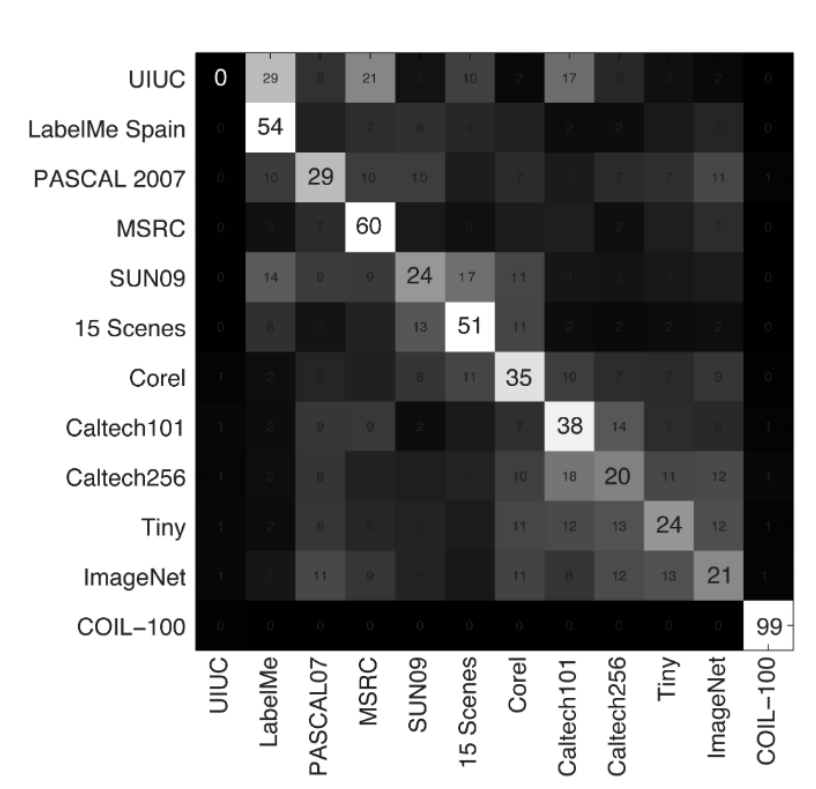
\includegraphics[width=\textwidth]{img/introduction/dataset_bias_confusion.png}
    \end{subfigure}
    \hspace{1cm}
    \begin{subfigure}[b]{0.32\textwidth}
        \centering
        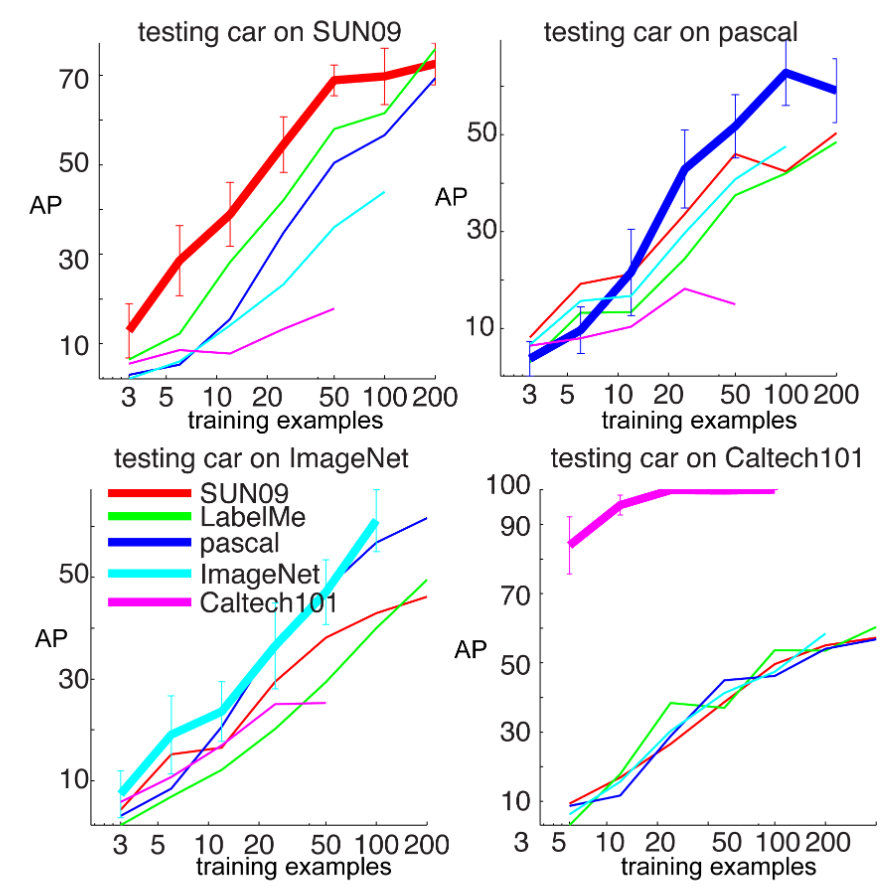
\includegraphics[width=\textwidth]{img/introduction/dataset_bias_cross_generalization.png}
    \end{subfigure}
       \caption{
        \textbf{(left)} Confusion matrix generated in a dataset
        identification task. A clearly pronounced diagonal 
        indicates that each dataset posesses unique traits that
        make it distinguishable from the rest.
        \textbf{(right)} Cross-dataset generalization
        for \texttt{car} detection as function of training data. 
        The vertical gap between lines represents the decrease in performance 
        when training on a different dataset, and the horizontal 
        shift corresponds to the increase in the amount of data needed 
        to reach the same performance.
        \cite{torralbaUnbiasedLookDataset2011}}
       \label{fig:dataset_bias}
\end{figure}

Several approaches can be taken to address this issue, depending
on the nature of the shift and the accessibility of the
causal structure of the data (see Figure 3 and Table 2 in 
\cite{wangGeneralizingUnseenDomains2022}).
Nevertheless, the common goal is to push the model towards
domain-invariant representations that foster robustness in the
face of distribution shifts, sometimes relaxing the causality condition
to an assumption of invariance or stability of the distribution in the output space
\cite{wangGeneralizingUnseenDomains2022,liuOutOfDistributionGeneralizationSurvey2023}. \\

In general, every formulation considers a set of source domains 
encompassing data that is available for the training of the model,
including any validation subsets used for model selection, 
regularization, or other hyperparameter tuning, and a set of target 
domains encompassing unseen data on which model performance will
be evaluated. Within this framework, a straightforward approach
to improving robustness is to directly sample target domains
and adjust feature representations to be invariant 
between both, which is known as domain adaptation. \\

In this work we will focus instead on domain generalization, which 
refers to the case in which target domains are not accessible 
and feature invariance can be only enforced 
from the source
\cite{blanchardGeneralizingSeveralRelated}. In particular, two strategies will be considered, 
namely domain alignment and data augmentation/generation. \\

On the one hand, domain alignment stems from the target invariance hypothesis, 
and can be formulated as a regularization problem that pushes towards the 
minimization of the dissimilarity of feature  representations originated 
from different source environments. The feature space in which the 
alignment is performed (e.g. kernel latent space 
\cite{muandetDomainGeneralizationInvariant2013}, 
adversarial
\cite{peiMultiAdversarialDomainAdaptation}
or model-based
\cite{arjovskyInvariantRiskMinimization2020}) 
and the similarity metric will
determine the the particularities of the method
\cite{shenWassersteinDistanceGuided2018,liangComprehensiveSurveyTestTime2023}. \\

\begin{figure}[H]
    \centering
    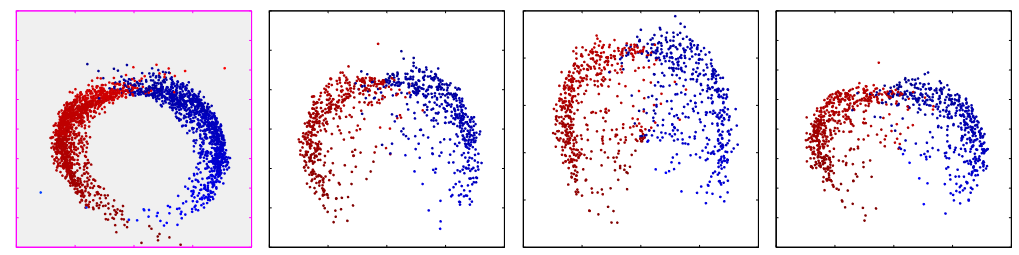
\includegraphics[width=0.65\textwidth]{img/introduction/dica.png}
    \caption{
    Projections of a binary synthetic dataset in the two principal DICA
    dimensions. The shaded box depicts the projection of training 
    data, whereas the unshaded boxes show projections of unseen 
    test datasets. \cite{muandetDomainGeneralizationInvariant2013}
    }
    \label{fig:dica}
\end{figure}

\begin{figure}[H]
    \centering
    \begin{subfigure}[b]{0.2\textwidth}
        \centering
        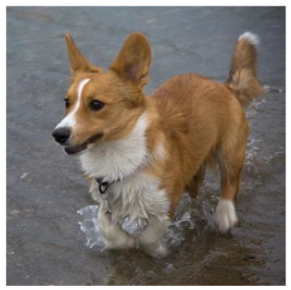
\includegraphics[width=\textwidth]{img/introduction/da_original.png}
        \caption{Original}
    \end{subfigure}
    \hspace{1cm}
    \begin{subfigure}[b]{0.2\textwidth}
        \centering
        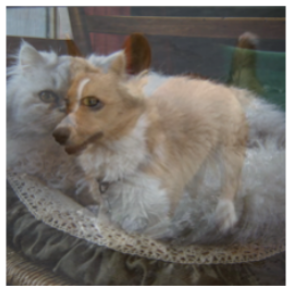
\includegraphics[width=\textwidth]{img/introduction/da_mixup.png}
        \caption{Mixup 
        \cite{zhangMixupEmpiricalRisk2018}
        }
    \end{subfigure}
    \hspace{1cm}
    \begin{subfigure}[b]{0.2\textwidth}
        \centering
        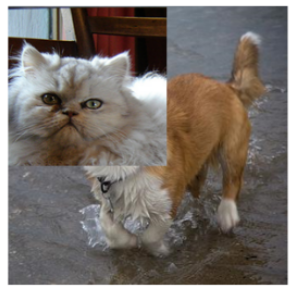
\includegraphics[width=\textwidth]{img/introduction/da_cutmix.png}
        \caption{CutMix
        \cite{yunCutMixRegularizationStrategy2019}
        }
    \end{subfigure}
       \caption{
        Mixup and Cutmix strategies can be used to interpolate
        between different labels and/or domains
        by generating intermediate observations.
        \cite{yunCutMixRegularizationStrategy2019}
        }
       \label{fig:data_augmentation}
\end{figure}

On the other hand, data augmentation/generation strategies 
do not need to assume target invariance and instead 
achieve cross-domain generalization by generating new samples that
diversify the original dataset with the hope of capturing 
the underlying causal structure of the data generation process. Augmented samples
can either be randomizations of original observations (e.g. transformations
such as rescaling or rotations) or new samples filling the distribution
gaps between domains, as illustrated in Figure \ref{fig:data_augmentation}. \\

Unlike in the adversarial setting, there is no common way of measuring
the shift in distribution betweeen source domains, and current approaches
are often constrained to specific datasets or training strategies. 
Robustness is instead quantified during (cross-)validation, either by reserving
a subset of each domain, leaving one domain out, or
by directly accessing target domains if they are available, 
which is known as the oracle approach. This last strategy is often
used to provide an upper bound estimate of model robustness, 
as it usually provides over-confident performance estimates
\cite{zhouDomainGeneralizationSurvey2022}.
Numerous benchmark datasets, some of which will be considered in this work, are the current 
standard for robustness assessment even with
the limitations they present
\cite{kohWILDSBenchmarkIntheWild2021}. 
\\

%Despite extensive research on the field and a wide variety
%of strategies envisionated, robustness to distribution shifts 
%continues to pose a fundamental challenge in machine learning. As
%previously mentioned, this difficulty primarily arises from the 
%violation of the sampling uniformity assumption, which renders 
%conventional learning techniques ineffective, and also from the 
%lack of a universal formal characterization of distribution shifts.
%Existing benchmark datasets, some of which will be considered in this work, are the current 
%standard for robustness assessment even with
%the limitations they present. \\

\section{Related work}

In the adversarial front, early work 
\cite{szegedyIntriguingPropertiesNeural2014}
unveiled the nature of the susceptibility of deep learning 
models to adversarial examples and FGSM 
\cite{goodfellowExplainingHarnessingAdversarial2015}
was introduced as an intuitive
approach for model regularization. 
Since then, several gradient-based methods have been
proven to enhance adversarial robustness, such as PGD
\cite{madryDeepLearningModels2019}, C\&W 
\cite{carliniEvaluatingRobustnessNeural2017},
FMN
\cite{pintorFastMinimumnormAdversarial2021} and
many others (see 
\cite{liReviewAdversarialAttack2022} for reference). 
All of them ultimately entail a strategy to find
a vulnerable direction and adjust the perturbation 
(e.g. minimum-norm, maximum-confidence, etc.)
based on the location of the decision boundary, either via soft
constraints (i.e. regularization), boundary attacks or gradient
projections
\cite{baiRecentAdvancesAdversarial2021}. \\

In general, the primary distinction among adversarial attacks lies in
their knowledge of the model's architecture and parameters. In that
sense, white-box and black-box
attacks can be distinguished, where the former have full 
access to the model and the latter only 
to the model's predictions. In black-box settings the loss gradient
is unknown and other strategies such as score-based or
decision-based attacks are used
\cite{liReviewAdversarialAttack2022}. Regarding adversarial training (i.e. defenses), 
robustness can
be achieved by a variety of methods, 
such as ensemble learning,
defensive distillation,
generative adversarial networks
\cite{xiaoGeneratingAdversarialExamples2019, miyatoVirtualAdversarialTraining2018},
diffusion models
\cite{wangBetterDiffusionModels2023,hoDenoisingDiffusionProbabilistic2020}
and adaptive-boundary methods
\cite{cohenCertifiedAdversarialRobustness2019}.
In this project, the Robustbench attack library
\cite{croceRobustBenchStandardizedAdversarial2021a}
will be used for adversarial robustness evaluation 
in the \texttt{CIFAR10} dataset
\cite{krizhevskyLearningMultipleLayers}. \\

In the domain generalization front, the existing rich taxonomy 
of methods can be classified into three main groups, namely
data manipulation, representation learning 
and alternative learning strategies
\cite{wangGeneralizingUnseenDomains2022,zhouDomainGeneralizationSurvey2022,liuOutOfDistributionGeneralizationSurvey2023}.
Data manipulation strategies refer to augmentation and generation,
as for example randomization or adversarial augmentation
\cite{yaoImprovingOutofDistributionRobustness2022,zhangMixupEmpiricalRisk2018,yunCutMixRegularizationStrategy2019}.
Representation learning strategies are primarily divided 
into domain-invariant methods (e.g. IRM
\cite{arjovskyInvariantRiskMinimization2020} or
kernel-based
\cite{muandetDomainGeneralizationInvariant2013,arjovskyWassersteinGAN2017}) 
and feature disentanglement methods, which encompass causality-inspired
approaches and general multi-component analysis. Other 
learning strategies include meta-learning
\cite{liLearningGeneralizeMetaLearning2018,wangMetaFineTuningNeural2020},
ensemble learning or self-supervised learning. \\

Regarding robustness characterization, a wide range of metrics
have been conceived (see
\cite{guoComprehensiveEvaluationFramework2023} for reference), but
accuracy-based criteria are still the most common. Alternatively, 
some  theoretically-grounded approaches have been proposed, such
as CLEVER \cite{wengEvaluatingRobustnessNeural2018}, ACTS 
\cite{wangGeometricalApproachEvaluate2023}
or
PA
\cite{buhmannPosteriorAgreementModel2022}, 
which is the one explored in this work. 
In general, robustness is often reported and compared using 
robustness benchmark datasets. Some of the most relevant
for image classification tasks are 
MNIST (and its multiple variations, such as DiagVib-6
\cite{euligDiagViB6DiagnosticBenchmark2021}),
PACS
\cite{yuPACSDatasetPhysical2022},
VLCS
\cite{khoslaUndoingDamageDataset2012}
or WILDS
\cite{kohWILDSBenchmarkIntheWild2021}.

\section{Objectives}

The main goal of this project is to assess
the suitability of the posterior agreement framework in the 
context of deep learning model robustness for image 
classification tasks. For that, an operative version of posterior
agreement for finite, discrete hypothesis classes must be derived and
efficiently implemented, so that it can be used as a metric to evaluate 
and select models based on the robustness of their response to different 
sources and levels of randomness. The results obtained should be compared
with the current state-of-the-art in robustness evaluation, namely
Robustbench
\cite{croceRobustBenchStandardizedAdversarial2021a}
and WILDS 
\cite{kohWILDSBenchmarkIntheWild2021}
benckmarks in the adversarial and
out-of-distribution settings, respectively, and an overall
analysis of the use of the metric as an early-stopping 
criterion should be provided.\\

In order to conduct a comprehensive assessment, a series of steps should be undertaken in a 
deductive manner, so that evidence is provided starting from first principles and culminating
with performance evaluations on benchmark datasets. To begin with, the content of this work should
be self-contained, and for that a formal statement of the learning problem should be given. Both 
learning algorithms and classification models should be defined, including the nuances of their
parametrization via deep neural networks. \\

Next, the robustness challenge should be formulated within the framework of probability theory,
providing a rigorous mathematical foundation for understanding the principal sources of randomness that
are relevant in the context of this work. The generalization capabilities to specific sources of randomness
will determine the robustness score of a model, which for PA is conceived as a 
measure of the stability of the probabilistic output of the model to the randomness of the data 
sampling process. In this sense, the fundamental generalization-complexity trade-off must be reframed
within the context of information theory by relating complexity to the expected information content
of the data. The estimated informativeness will determine the resolution of the hypothesis space and
thus its stability under perturbations of various kinds. Once an operative PA metric is derived, 
its properties should be investigated and further assessed with artificial data, so that PA can be compared 
with baseline accuracy-based metrics at a fundamental level. \\

Experiments should be performed the adversarial setting first, for being adversarial perturbations
intentionally designed to change the prediction of the model and thus entailing a performance-based notion of
robustness that aligns with accuracy measures. After that, a customized implementation of 
the DiagVib-6 
\cite{euligDiagViB6DiagnosticBenchmark2021} 
syntetic data generation pipeline should be used to evaluate the suitability of PA in the domain
generalization setting. This will allow for a detailed analysis of the model selection capabilities of PA 
under different experimental conditions, especially regarding the source, power and rate of the shift 
entailed by each dataset and the accessibility of target domains for model validation and selection.\\


All in all, both analytical and numerical tools should be used to provide a comprehensive analysis
of the model-selection capabilities of PA and the source of its discriminative power. \\




